%Author Cesar
%Desc : For my presentations


\documentclass{beamer}\usetheme{Madrid} %

\setbeamercovered{invisible} % To remove the navigation symbols from
% the bottom of slides%
%\setbeamertemplate{navigation symbols}{}  %Disable the navigation
%

\usepackage{upquote} %proper quotation inside the verbatim

% sudo apt-get install texlive-full or texlive-science (the latter is minimal)
\usepackage{algorithmic}
\usepackage{amsmath}
\usepackage{mathtools}
\usepackage{amssymb}

\usepackage[spanish]{babel} 
\usepackage{algorithm2e}
\usepackage{multicol}
\usepackage{xcolor}
\usepackage{fancyvrb}
\usepackage{listings}
\usepackage{boxedminipage} %modified Madrid footer
\usepackage{graphicx}
\usepackage{caption}
\usepackage[utf8]{inputenc}
%\usepackage{bm}         % For typesetting bold math (not \mathbold)
%\logo{\includegraphics[height=0.6cm]{yourlogo.eps}}


\title[ACR]{Refinamiento Adaptivo de Código}
\author{C\'esar Sabater} \institute[UNR] {
%University of Strasbourg \\

\medskip
%{\emph{aravind.sukumaran-rajam@inria.fr}}\\
%\vspace{10px}

\includegraphics[scale=0.1]{img/logo.png} }

\subject{ Presentaci\'on de Tesina } % \tiny{ }

\date{ \today} % \today will show
%current date.

\setbeamertemplate{navigation symbols}{}%remove navigation symbols 

%custom beaver footnote do what ever u want
\setbeamertemplate{footline} {%
\leavevmode
%
\hbox{%
\begin{beamercolorbox}[wd=.323\paperwidth,ht=2.25ex,dp=1ex,center]
    {author in head/foot}%
    \usebeamerfont{author in head/foot} Universidad Nacional de Rosario
\end{beamercolorbox}
%
\begin{beamercolorbox}[wd=.333\paperwidth,ht=2.25ex,dp=1ex,center]
    {title in head/foot}%
    \usebeamerfont{title in head/foot}\insertshorttitle
\end{beamercolorbox}
%
\begin{beamercolorbox}[wd=.3333\paperwidth,ht=2.25ex,dp=1ex,right]
    {date in head/foot}%
    \usebeamerfont{date in head/foot}\insertshortdate{}\hspace*{2em}
    \insertframenumber{} / \inserttotalframenumber\hspace*{1ex}
\end{beamercolorbox}
}%
\vskip0pt%
}

%\logo{
\includegraphics[scale=.04]{img/logo.png}}

\newcommand\codeHighlight[1]{\textcolor[rgb]{1,0,0}{\textbf{#1}}}

%~ \newenvironment{rcases} {\left.
%~ \begin{aligned}
    %~ } {%
%~ \end{aligned}
%~ \right\rbrace}

\lstset{escapeinside={@@}{@^}}

\begin{document}
%
{ \setbeamertemplate{logo}{}
\begin{frame}
    \titlepage
    \vspace*{-25px}
    \begin{center}
        \large{ Presentaci\'on de Tesina }
    \end{center}
\end{frame}
}

%%%%%%%%%%%%%%%%%%%%%%%%%%%%%%%%%%%%%%%%%%%%%%%%%%%%%%%%%%%%%%%%%%%%%%%%%%%%%%%%
\begin{frame}
    \frametitle{Introducción}
    %more concrete simualtions, but a more abstract kind of problem
    \begin{itemize}
    \item
    Muchas aplicaciones de \textbf{cómputo intensivo} realizan
    \textbf{cálculos aproximados}
    \item 
    Algunas Razones: 
    \begin{itemize}
        \item
			para simular objetos o fenómenos del mundo real
		\item
			trabajan con sensores limitados en precisión
		\item
			están sometidas a un deadline de tiempo
		\item
			calculan resultados preliminares
    \end{itemize}
    \end{itemize}
\end{frame}
%%%%%%%%%%%%%%%%%%%%%%%%%%%%%%%%%%%%%%%%%%%%%%%%%%%%%%%%%%%%%%%%%%%%%%%%%%%%%%%%
\begin{frame}
\frametitle{Introducción}
Algunos ejemplos de estas aplicaciones son: 
    \begin{itemize}
        \item
			Simulaciones Físicas
		\item
			Sensores de entrada, algoritmos de procesamiento
		\item
			Decodificación de Video en tiempo real
		\item 
			Predicción de Terremotos
		\item 
			Aplicaciones de exploración de geofísica
    \end{itemize}
    %~ Generalmente, estas aplicaciones necesitan una gran cantitdad de poder computacional.
   %~ \begin{figure} 
	 %~ 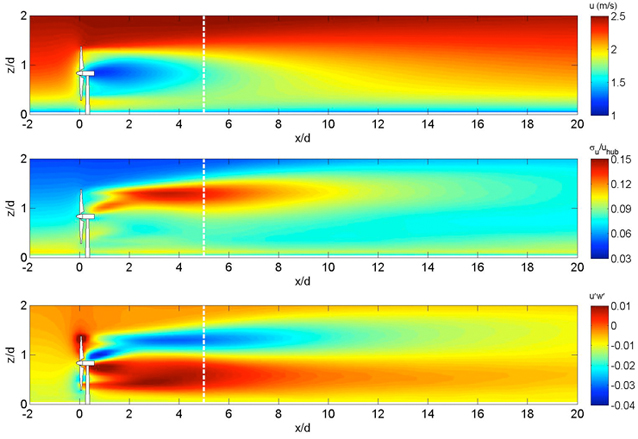
\includegraphics[scale=0.18]{img/wind_sim.jpg}
    %~ \end{figure}
\end{frame}
%%%%%%%%%%%%%%%%%%%%%%%%%%%%%%%%%%%%%%%%%%%%%%%%%%%%%%%%%%%%%%%%%%%%%%%%%%%%%%%%
\begin{frame}
\frametitle{Introducción}
Normalmente, el desarrollo de estos 
algoritmos puede dividirse en \textbf{dos etapas}:
\begin{itemize}
\item Desarrollo de un kernel de computo ideal
	\begin{itemize} 
	\item ajuste del algoritmo
	\item debugueo
	\end{itemize}
\item Optimización a una versión de producción
	\begin{itemize}
	\item ajustando el nivel de precisión para realizar cálculos
	precisos solo donde es necesario
	\item escalar al tamaño real del problema
	\item satisfacer un deadline
	\end{itemize}
\end{itemize}
\end{frame}
%%%%%%%%%%%%%%%%%%%%%%%%%%%%%%%%%%%%%%%%%%%%%%%%%%%%%%%%%%%%%%%%%%%%%%%%%%%%%%%%
\begin{frame}
\frametitle{Introducción}
Optimizar un kernel ideal tiene complicaciones: 
\begin{itemize} 
\item es \textcolor{red}{complejo}
\item \textcolor{red}{lleva tiempo}
\item conduce a \textcolor{red}{códigos menos mantenibles}
\item hay que \textcolor{red}{hacerlo nuevamente} cuando hay cambios grandes en la estrategia
\end{itemize}
Esto se podría reducir con un \textbf{enfoque automático de compilación}
\end{frame}
%%%%%%%%%%%%%%%%%%%%%%%%%%%%%%%%%%%%%%%%%%%%%%%%%%%%%%%%%%%%%%%%%%%%%%%%%%%%%%%%
\begin{frame}
\frametitle{Introducción}
	Existen enfoques automáticos de optimización para computo intensivo:
	\begin{itemize}
	\item manteniendo la semántica original
	\begin{itemize}
		\item paralelización
		\item localidad de datos
		\item vectorización
	\end{itemize}
	\textcolor{blue}{bien abordados por los compiladores}
	\item modificando la semántica original
	\begin{itemize}
		\item relajación de dependencias
		\item modificación o eliminación de cálculos
		\item usando conocimiento especifico de dominio 
	\end{itemize} 
	\textcolor{red}{escasamente abordados por los compiladores}
	\end{itemize}
\end{frame}
%%%%%%%%%%%%%%%%%%%%%%%%%%%%%%%%%%%%%%%%%%%%%%%%%%%%%%%%%%%%%%%%%%%%%%%%%%%%%%%%
\begin{frame}
\frametitle{Introducción}

Para aplicaciones que calculan resultados aproximados, un enfoque automático 
de optimización que modifique la semántica original es adecuado siempre
que asegure una \textbf{precisión aceptable}.

\end{frame} 
%%%%%%%%%%%%%%%%%%%%%%%%%%%%%%%%%%%%%%%%%%%%%%%%%%%%%%%%%%%%%%%%%%%%%%%%%%%%%%%%
\begin{frame}
\frametitle{Introducción}
\textbf{Nuestro Objetivo}: Buscar formas de optimizar códigos que computan
aproximaciones 
\begin{itemize} 
\item de forma \textbf{automática}
\item \textbf{modificando la semántica} original
\item asegurando una \textbf{precisión aceptable} 
\end{itemize}
\end{frame}
%%%%%%%%%%%%%%%%%%%%%%%%%%%%%%%%%%%%%%%%%%%%%%%%%%%%%%%%%%%%%%%%%%%%%%%%%%%%%%%%
\begin{frame}
\frametitle{Introducción}
Para realizarlo utilizaremos
\begin{itemize} 
\item El \textbf{Modelo Poliédrico} para realizar transformaciones agresivas de código
\item \textbf{Conocimiento de Dominio Especifico} suministrado por el usuario
	\begin{itemize} 
	\item que guíe la transformación de código	
	\item mantenga una precisión aceptable
\end{itemize}
\item Un enfoque \textbf{adaptivo}
	\begin{itemize} 
		\item realiza cálculos complejos solamente donde es necesario
		\item ahorra computaciones que no impactan en el resultado
		\item transforma el código de forma dinámica
	\end{itemize}
\end{itemize}
\end{frame}
%%%%%%%%%%%%%%%%%%%%%%%%%%%%%%%%%%%%%%%%%%%%%%%%%%%%%%%%%%%%%%%%%%%%%%%%%%%%%%%%
\begin{frame} 
\frametitle{Contenido} 
\begin{enumerate}
\item \textbf{Transformación de Código: Modelo Poliédrico}
\item Herramienta estática: Spot
\item Refinamiento Adaptivo de Código
\item Experimentos con Simulación de Fluidos
\item Conclusiones y Trabajo Futuro
\end{enumerate}
\end{frame} 
%%%%%%%%%%%%%%%%%%%%%%%%%%%%%%%%%%%%%%%%%%%%%%%%%%%%%%%%%%%%%%%%%%%%%%%%%%%%%%%%
\begin{frame} 
\frametitle{Modelo Poliédrico}
	\begin{itemize} 
	\item Es un modelo matemático-computacional para la optimización y 
			paralelización automática de programas
	\item muy poderoso para la representación y transformación estructural de programas
	\item Representa bucles matemáticamente con \textbf{relaciones afines}
		\begin{itemize}
		\item dominios de iteración
		\item relaciones de orden
		\item relaciones de acceso
		\end{itemize}
	\end{itemize}
		\begin{figure}
			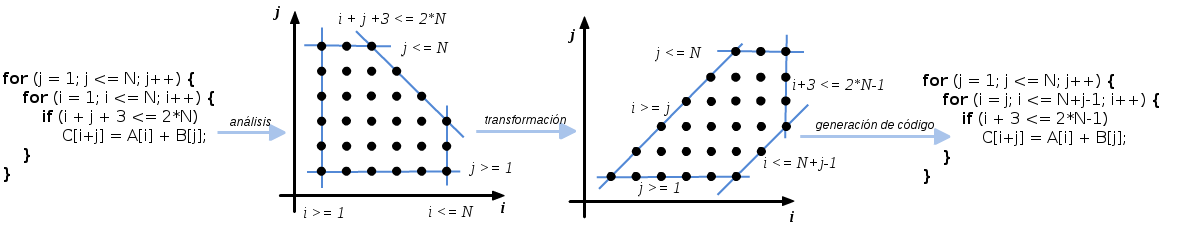
\includegraphics[scale=0.30]{img/poly_pipeline2.png}
		\end{figure}
\end{frame}
%%%%%%%%%%%%%%%%%%%%%%%%%%%%%%%%%%%%%%%%%%%%%%%%%%%%%%%%%%%%%%%%%%%%%%%%%%%%%%%%
\begin{frame}[fragile]
\frametitle{Dominios de Iteración}
\begin{itemize}
\item \textbf{instancia de statement}: una ejecución individual de un statement $S$ 
\item $S(i',j')$ es la instancia de $S$ para los valores $i=i'$ y $j=j'$ 
\item el \textbf{dominio de iteración} queda definido por el conjunto de valores
del vector $\left(\begin{smallmatrix}i\\j\\\end{smallmatrix}\right)$
\item el dominio de iteración se puede representar con \textbf{poliedros} 
\end{itemize}
\begin{columns}
\column[t]{0.55\textwidth}
%~ \begin{figure}
\begin{block}{multiplicacion de polinomios}
\begin{lstlisting}[basicstyle=\scriptsize,language=C]
    for (i = 0; i < 2 * N - 1; i++) 
S1:     z[i] = 0;
        
    for (i = 0; i < N; i++) 
        for (j = 0; j < N; j++)
S2:         @@\textcolor{violet}{z[i+j] = x[i] + y[j];} @^
\end{lstlisting}
\end{block}
%~ \caption{multiplicación de matrices}
%~ \end{figure}
\column[t]{0.45\textwidth}
\begin{figure}
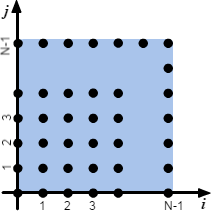
\includegraphics[scale=0.4]{img/poly_mul_solo.png}
\caption{instancias de $S2$}
\end{figure}
\end{columns}
\end{frame}
%%%%%%%%%%%%%%%%%%%%%%%%%%%%%%%%%%%%%%%%%%%%%%%%%%%%%%%%%%%%%%%%%%%%%%%%%%%%%%%%
\begin{frame}
\frametitle{Representación poliédrica: Dominios de Iteración}
\begin{columns}
\column[t]{0.45\textwidth}
inecuaciones del dominio de iteración de $S2$: 
\begin{itemize}
\item $ i \geq 0 $
\item $ i  < N $
\item $ j \geq 0 $
\item $ j < N $
\end{itemize}
\column[t]{0.45\textwidth}
ecuación matricial: 
$$
\begin{bmatrix*}[r] 1 &  0 & 0 &  0 \\ 
                               -1 &  0 & 1 & -1 \\ 
                                0 &  1 & 0 &  0 \\
                                0 & -1 & 1 & -1 \end{bmatrix*} 
            \left( \begin{array}{c} i \\ j \\ N\\ 1\\ \end{array} \right)
            \geq \vec{0}
$$
\end{columns}
\begin{itemize}
\item representación \textcolor{blue}{poderosa y compacta} 
\item \textcolor{red}{restricciones}:
\begin{itemize}
\item no hay esquema general para soportar flujo de control dinámico
\item cotas de bucles y condicionales \textcolor{red}{deben ser funciones afines}
de iteradores exteriores y parámetros
\end{itemize}
\end{itemize} 
\end{frame}
%%%%%%%%%%%%%%%%%%%%%%%%%%%%%%%%%%%%%%%%%%%%%%%%%%%%%%%%%%%%%%%%%%%%%%%%%%%%%%%%
\begin{frame}[fragile]
\frametitle{Representación poliédrica: Relaciones de Ordenamiento}
\begin{itemize}
\item especifican \textbf{orden temporal y espacial} de cada instancia
\item \textbf{temporal}: momento de ejecución de una instancia ejecución con respecto
a las otras
\item \textbf{espacial}: procesador asignado 
\item a cada instancia se le asigna una \textbf{fecha lógica}
\begin{columns}
\column[t]{0.40\textwidth}
\begin{equation}
\nonumber
\theta_{S_1}(N, i) = \left(\begin{matrix} 0 \\ i\\\end{matrix} \right)
\end{equation}
\begin{equation}
\nonumber
\theta_{S_2}(N, i, j) =  \left(\begin{matrix} 1 \\ i \\ j \\\end{matrix} \right)
\end{equation}
\column[t]{0.55\textwidth}
%~ \begin{figure}
\begin{block}{multiplicacion de polinomios}
\begin{lstlisting}[basicstyle=\scriptsize,language=C]
    for (i = 0; i < 2 * N - 1; i++) 
S1:     z[i] = 0;
        
    for (i = 0; i < N; i++) 
        for (j = 0; j < N; j++)
S2:         z[i+j] = x[i] + y[j];
\end{lstlisting}
\end{block}
%~ \end{figure}
\vfill \null
\end{columns}
\item los statements se ejecutan en \textcolor{blue}{orden lexicográfico} 
\item si poseen la misma fecha lógica \textcolor{blue}{pueden ser ejecutados en paralelo}
\item \textcolor{red}{las funciones de ordenamiento deben ser afines}
\end{itemize}
\end{frame}
%%%%%%%%%%%%%%%%%%%%%%%%%%%%%%%%%%%%%%%%%%%%%%%%%%%%%%%%%%%%%%%%%%%%%%%%%%%%%%%%
\begin{frame}
\frametitle{Representación poliédrica: Relaciones de Ordenamiento}
relaciones afines: 
$$
{\scriptstyle
 \theta_{S_1}(N) = 
        \left\{ 
            \left(\begin{matrix}i\\\end{matrix} \right) \to 
            \left(\begin{matrix}t_1 \\ t_2\\\end{matrix} \right) 
            \in \mathbb{Z} \times \mathbb{Z}^2  \middle|
            \begin{bmatrix*}[r] -1 &  0 & 0 &  0 & 0 \\ 
                                0  & -1 & 1 &  0 & 0  \end{bmatrix*} 
            \left( \begin{array}{c} t_1 \\ t_2 \\ i \\ N \\ 1\\ \end{array} \right)
            = \vec{0}
        \right\},
}
$$ 
$$
{\scriptstyle
 \theta_{S_2}(N) = 
        \left\{ 
            \left(\begin{matrix}i \\ j \\\end{matrix} \right) \to 
            \left(\begin{matrix}t_1 \\ t_2 \\ t_3 \\\end{matrix} \right) 
            \in \mathbb{Z}^2 \times \mathbb{Z}^3  \middle|
            \begin{bmatrix*}[r] -1 &  0 &  0 & 0 &  0 & 0 & 1 \\ 
                                0  & -1 &  0 & 1 &  0 & 0 & 0 \\
                                0  &  0 & -1 & 0 &  1 & 0 & 0 \end{bmatrix*} 
            \left( \begin{array}{c} t_1 \\ t_2 \\ t_3 \\ i \\ j \\ N \\ 1\\ \end{array} \right)
            = \vec{0}
        \right\}
}
$$
\end{frame}
%%%%%%%%%%%%%%%%%%%%%%%%%%%%%%%%%%%%%%%%%%%%%%%%%%%%%%%%%%%%%%%%%%%%%%%%%%%%%%%%
\begin{frame}[fragile]
\frametitle{Representación Poliédrica: Funciones de Acceso}
\begin{itemize}
\item modelan accesos a memoria
\item los accesos deben ser funciones afines de iteradores envolventes
y parámetros fijos
\end{itemize}
\begin{columns}
\column[t]{0.40\textwidth}
\begin{equation}
\nonumber
A_{{S_1},1}(N, i) = \left(\begin{matrix} i\\\end{matrix} \right)
\end{equation}
\begin{equation}
\nonumber
A_{{S_2},2}(N, i, j) =  \left(\begin{matrix} i + j \\\end{matrix} \right)
\end{equation}
\begin{equation}
\nonumber
A_{{S_2},3}(N, i, j) =  \left(\begin{matrix} i \\\end{matrix} \right)
\end{equation}
\begin{equation}
\nonumber
A_{{S_2},4}(N, i, j) =  \left(\begin{matrix} j \\\end{matrix} \right)
\end{equation}
\column[t]{0.55\textwidth}
\begin{block}{}
\begin{lstlisting}[basicstyle=\scriptsize,language=C]
    for (i = 0; i < 2 * N - 1; i++) 
S1:     z[i] = 0;
        
    for (i = 0; i < N; i++) 
        for (j = 0; j < N; j++)
S2:         z[i+j] = x[i] + y[j];
\end{lstlisting}
\end{block}
%~ \end{figure}
\vfill \null
\end{columns}
\end{frame}
%%%%%%%%%%%%%%%%%%%%%%%%%%%%%%%%%%%%%%%%%%%%%%%%%%%%%%%%%%%%%%%%%%%%%%%%%%%%%%%%

\begin{frame}
\frametitle{Representación Poliédrica: Funciones de Acceso}
$$
{\scriptstyle
 A_{S_1,1}(N) = 
        \left\{ 
            \left(\begin{matrix}i\\\end{matrix} \right) \to 
            \left(\begin{matrix} a_{S_1,1} \\\end{matrix} \right) 
            \in \mathbb{Z} \times \mathbb{Z}  \middle|
            \begin{bmatrix*}[r] -1 & 1 & 0 & 0 \end{bmatrix*} 
            \left( \begin{array}{c} a_{S_1,1} \\ i \\ N \\ 1\\ \end{array} \right)
            = \vec{0}
        \right\},
}
$$
$$
{\scriptstyle
 A_{S_2,1}(N) = 
        \left\{ 
            \left(\begin{matrix}i \\ j \\\end{matrix} \right) \to 
            \left(\begin{matrix} a_{S_2,1} \\\end{matrix} \right) 
            \in \mathbb{Z}^2 \times \mathbb{Z}  \middle|
            \begin{bmatrix*}[r] -1 & 1 & 1 & 0 & 0 \\ \end{bmatrix*} 
            \left( \begin{array}{c} a_{S_2,1} \\ i \\ j \\ N \\ 1\\ \end{array} \right)
            = \vec{0}
        \right\},
}
$$
\end{frame}
%%%%%%%%%%%%%%%%%%%%%%%%%%%%%%%%%%%%%%%%%%%%%%%%%%%%%%%%%%%%%%%%%%%
\begin{frame}
\frametitle{Representación Poliédrica: Funciones de Acceso}
$$
{\scriptscriptstyle
 A_{S_2,2}(N) = 
        \left\{ 
            \left(\begin{matrix}i \\ j \\\end{matrix} \right) \to 
            \left(\begin{matrix} a_{S_2,2} \\\end{matrix} \right) 
            \in \mathbb{Z}^2 \times \mathbb{Z}  \middle|
            \begin{bmatrix*}[r] -1 & 1 & 0 & 0 & 0 \\ \end{bmatrix*} 
            \left( \begin{array}{c} a_{S_2,2} \\ i \\ j \\ N \\ 1\\ \end{array} \right)
            = \vec{0}
        \right\},
}
$$
$$
{\scriptscriptstyle
 A_{S_2,3}(N) = 
        \left\{ 
            \left(\begin{matrix}i \\ j \\\end{matrix} \right) \to 
            \left(\begin{matrix} a_{S_2,3} \\\end{matrix} \right) 
            \in \mathbb{Z}^2 \times \mathbb{Z}  \middle|
            \begin{bmatrix*}[r] -1 & 0 & 1 & 0 & 0 \\ \end{bmatrix*} 
            \left( \begin{array}{c} a_{S_2,3} \\ i \\ j \\ N \\ 1\\ \end{array} \right)
            = \vec{0}
        \right\}.
}
$$
\end{frame}
%%%%%%%%%%%%%%%%%%%%%%%%%%%%%%%%%%%%%%%%%%%%%%%%%%%%%%%%%%%%%%%%%%%%%%%%%%%%%%%%
\begin{frame}
\frametitle{Modelo Poliédrico: Transformaciones}
\textbf{transformaciones}
\begin{itemize}
	\item relaciones de ordenamiento
	\item dominios de iteración
	%~ \item relaciones de acceso
	\item \textcolor{red}{mantienen la semántica} si respetan las dependencias de datos
	\begin{itemize}
		\item mantener el orden de instancias \textbf{en relación de dependencia}
		\begin{itemize}
			\item acceden a los mismos datos
			\item RAW, WAR, WAW
			\item RAR no es técnicamente dependencia, pero es bueno para la localidad
		\end{itemize}
	\end{itemize}
\end{itemize}
\begin{figure}
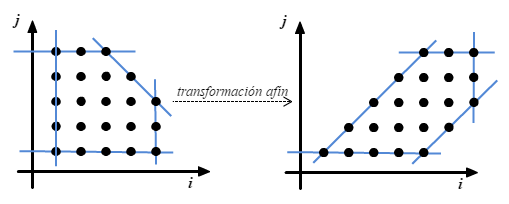
\includegraphics[scale=0.6]{img/poly_transf.png}
\end{figure}
\end{frame}
%%%%%%%%%%%%%%%%%%%%%%%%%%%%%%%%%%%%%%%%%%%%%%%%%%%%%%%%%%%%%%%%%%%%%%%%%%%%%%%%
\begin{frame}
\frametitle{Modelo Poliédrico: Generación de Código}
\textbf{generación de código}
\begin{itemize}
\item problema: \textbf{encontrar un código eficiente que visite todos los puntos de un poliedro respetando el orden lexicográfico}
\item se traduce a un problema de \textbf{escaneo de poliedros}
\begin{itemize}
\item basada eliminación Fourier-Motzkin
\item programación entera perimétrica
\item método de \textbf{Quilleré, Rajopadhye y Wilde}
\end{itemize}
\item extensiones de \textbf{QRW} generan códigos con \textcolor{blue}{bajo costo de control}
\end{itemize}
\end{frame}
%%%%%%%%%%%%%%%%%%%%%%%%%%%%%%%%%%%%%%%%%%%%%%%%%%%%%%%%%%%%%%%%%%%%%%%%%%%%%%
\begin{frame}
\frametitle{Modelo Poliédrico: Herramientas}
Las herramientas de compilación poliédrica que utilizamos son: 
\begin{itemize}
\item \textbf{OpenScop}
\begin{itemize}
\item formalismo para la representación de elementos del modelo poliédrico
\item conjunto de librerías para manipular estos elementos
\end{itemize}
\item \textbf{Clan}: transforma código a su representación poliédrica
\item \textbf{Cloog}: generación del código con el método QRW
\item \textbf{isl}: manipulación eficiente de conjuntos de enteros
\end{itemize}
\end{frame}
%%%%%%%%%%%%%%%%%%%%%%%%%%%%%%%%%%%%%%%%%%%%%%%%%%%%%%%%%%%%%%%%%%%%%%%%%%%%%
\begin{frame} 
\frametitle{Contenido} 
\begin{enumerate}
\item Transformación de Código: Modelo Poliédrico
\item \textbf{Herramienta estática: Spot}
\item Refinamiento Adaptivo de Código
\item Experimentos con Simulación de Fluidos
\item Conclusiones y Trabajo Futuro
\end{enumerate}
\end{frame} 
%%%%%%%%%%%%%%%%%%%%%%%%%%%%%%%%%%%%%%%%%%%%%%%%%%%%%%%%%%%%%%%%%%%%%%%%%%%%%%%%
\begin{frame} 
\frametitle{Spot}
\textbf{Spot}
\begin{itemize}
	\item \textbf{herramienta estática} de compilación
	\item permite al usuario \textbf{transformar} subconjuntos del dominio de iteración
	\begin{itemize}
		\item \textbf{reemplazando} bloques de código a ejecutar en cada instancia
		\item \textbf{ignorando} la ejecución de conjuntos de instancia
	\end{itemize}
	\item utiliza \textbf{pragmas especiales} para expresar matemáticamente sub-dominios de iteración 
\end{itemize}
\end{frame}
%%%%%%%%%%%%%%%%%%%%%%%%%%%%%%%%%%%%%%%%%%%%%%%%%%%%%%%%%%%%%%%%%%%%%%%%%%%%%%%%
\begin{frame}[fragile]
\frametitle{Spot: pragmas}
\begin{itemize}
	\item \textbf{entrada}: bucle anidado con \textcolor{blue}{pragmas} que denotan  \textbf{dominios~de~interés}
	\item los \textbf{pragmas} están compuestos por 
	\begin{itemize}
		\item un \textcolor{blue}{\textit{centinela}} \textcolor{blue}{\lstinline{\#pragma spot}}
		\item una \textcolor{purple}{\textit{prioridad}} mayor o igual a \lstinline{0}
		\item un \textcolor{olive}{\textit{dominio de interés}} en \textbf{\textbf{notación isl}}
		\item un \lstinline{bloque de statement}, si la \textcolor{purple}{\textit{prioridad}} es mayor a \lstinline{0} 
    \end{itemize}
%~ @@\textcolor{blue}{\#pragma spot}@^ 0 [N] -> {[i, j] | 0<=i<=3 and 0<=j<=3 }
%~ @@\textcolor{blue}{\#pragma spot}@^ 1 [N] -> {[i, j] | 5<=i<=8 and 2<=j<=9 } {A[i][j] = 1.11;} 
\begin{block}{}
\begin{lstlisting}[basicstyle=\scriptsize,language=C]
@@\textcolor{blue}{\#pragma spot} \textcolor{purple}{0} \textcolor{olive}{[N] -\textgreater \{ [i, j] \textbar  0\textless=i\textless=3 and 0\textless=j\textless=3\}}@^
@@\textcolor{blue}{\#pragma spot} \textcolor{purple}{1} \textcolor{olive}{[N] -\textgreater \{ [i, j] \textbar  5\textless=i\textless=8 and 2\textless=j\textless=9\}}@^ A[i][j] = 1.11; 
for (i = 0; i < N; i++) {
  for (j = 0; j < N; j++) {
    A[i][j] = 3.14;
  }
}
\end{lstlisting}
\end{block}
\item cuando la \textcolor{purple}{\textit{prioridad} es 0}, el sub-dominio \textbf{omitido de la ejecución}
\end{itemize}
\end{frame}
%%%%%%%%%%%%%%%%%%%%%%%%%%%%%%%%%%%%%%%%%%%%%%%%%%%%%%%%%%%%%%%%%%%%%%%%%%%%%%%%
\begin{frame}[fragile]
%~ \frametitle{Spot: salida}
\begin{columns}
\column[t]{0.38\textwidth}
\begin{block}{Salida Spot}
\begin{lstlisting}[basicstyle=\tiny,language=C]
if (N >= 5) {
  for (i=0;i<=3;i++) 
    for (j=4;j<=N-1;j++) 
      A[i][j] = 3.14;
  for (j=0;j<=N-1;j++) 
    A[4][j] = 3.14;
}
if (N >= 11) 
  for (i=5;i<=8;i++) {
    for (j=0;j<=1;j++) 
      A[i][j] = 3.14;
    for (j=2;j<=9;j++) 
      A[i][j] = 1.11;
    for (j=10;j<=N-1;j++) 
      A[i][j] = 3.14;
  }
if (N <= 10) 
  for (i=5;i<=min(8,N-1);i++) {
    for (j=0;j<=1;j++) 
      A[i][j] = 3.14;
    for (j=2;j<=9;j++) 
      A[i][j] = 1.11;
  }
for (i=9;i<=N-1;i++) 
  for (j=0;j<=N-1;j++) 
    A[i][j] = 3.14;
for (i=max(5,N);i<=8;i++) 
  for (j=2;j<=9;j++) 
    A[i][j] = 1.11;
\end{lstlisting}
\end{block}
\column[t]{0.6\textwidth}
\begin{itemize}
\item con \textbf{bloques de calculo alternativos} en los dominios de interés
con prioridad mayor a 0
\item \textbf{mayor prioridad} si hay dominios que se superponen
\item \textbf{omite cálculos} en regiones donde el nivel de interés es 0
\item \textbf{ejecuta cálculos originales} solo donde no hay dominios de interés
\item tiene \textbf{bajo costo de control}
\end{itemize}
\end{columns}
\end{frame}
%%%%%%%%%%%%%%%%%%%%%%%%%%%%%%%%%%%%%%%%%%%%%%%%%%%%%%%%%%%%%%%%%%%%%%%%%%%%%%%%
\begin{frame}[fragile]
\frametitle{Spot: Salida}
para \lstinline{N = 10}, con la matriz \lstinline{A} inicializada en \lstinline{0}
su estado final seria:
\begin{block}{Salida del Codigo Generado}
\begin{lstlisting}[basicstyle=\scriptsize] 
i/j 0     1     2     3     4     5     6     7     8     9
0   0.00  0.00  0.00  0.00  3.14  3.14  3.14  3.14  3.14  3.14 
1   0.00  0.00  0.00  0.00  3.14  3.14  3.14  3.14  3.14  3.14 
2   0.00  0.00  0.00  0.00  3.14  3.14  3.14  3.14  3.14  3.14 
3   0.00  0.00  0.00  0.00  3.14  3.14  3.14  3.14  3.14  3.14 
4   3.14  3.14  3.14  3.14  3.14  3.14  3.14  3.14  3.14  3.14 
5   3.14  3.14  1.11  1.11  1.11  1.11  1.11  1.11  1.11  1.11 
6   3.14  3.14  1.11  1.11  1.11  1.11  1.11  1.11  1.11  1.11 
7   3.14  3.14  1.11  1.11  1.11  1.11  1.11  1.11  1.11  1.11 
8   3.14  3.14  1.11  1.11  1.11  1.11  1.11  1.11  1.11  1.11 
9   3.14  3.14  3.14  3.14  3.14  3.14  3.14  3.14  3.14  3.14
\end{lstlisting}
\end{block}
\end{frame}
%%%%%%%%%%%%%%%%%%%%%%%%%%%%%%%%%%%%%%%%%%%%%%%%%%%%%%%%%%%%%%%%%%%%%%%%%%%%%%%%
\begin{frame}
\frametitle{Spot: Funcionamiento}
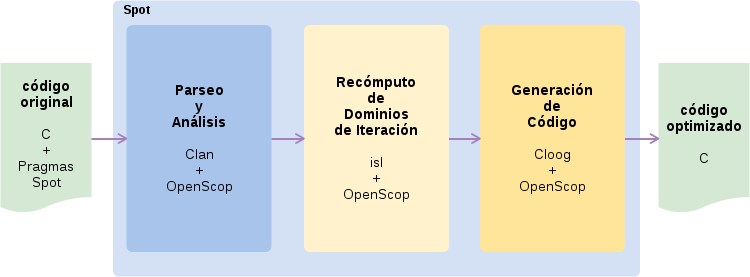
\includegraphics[scale=0.45]{img/spot_pipe_simple.png}
\end{frame}
%%%%%%%%%%%%%%%%%%%%%%%%%%%%%%%%%%%%%%%%%%%%%%%%%%%%%%%%%%%%%%%%%%%%%%%%%%%%%%%%
\begin{frame} 
\frametitle{Contenido} 
\begin{enumerate}
\item Transformación de Código: Modelo Poliédrico
\item Herramienta estática: Spot
\item \textbf{Refinamiento Adaptivo de Código}
\item Experimentos con Simulación de Fluidos
\item Conclusiones y Trabajo Futuro
\end{enumerate}
\end{frame} 
%%%%%%%%%%%%%%%%%%%%%%%%%%%%%%%%%%%%%%%%%%%%%%%%%%%%%%%%%%%%%%%%%%%%%%%%%%%%%%%%
\begin{frame}
\frametitle{Refinamiento Adaptivo de Código} 
\begin{block}{}
Técnica para la optimizacion \textbf{dinámica} y \textbf{automática} de programas que 
\textbf{computan aproximaciones}, a traves del \textbf{ahorro de calculos}.
\end{block}
En ingles, Adaptive Code Refinement $\rightarrow$ \textbf{ACR}
\begin{block}{Funcionamiento} 
ACR toma un codigo con \textbf{conocimiento de dominio} embebido
\begin{itemize}
	\item indica \textbf{estategias de ahorro de calculos}
	\item asegura \textbf{precision aceptable}
\end{itemize}
\textbf{transforma y ejecuta constantemente} versiones optimizadas del kernel
\begin{itemize}
	\item de forma \textbf{dinamica}s
	\item \textbf{adaptadas} a cada estado de la ejecucion
	\item realiza calculos complejos \textbf{solamente donde es necesario} 
\end{itemize}
\end{block}
\end{frame}
%%%%%%%%%%%%%%%%%%%%%%%%%%%%%%%%%%%%%%%%%%%%%%%%%%%%%%%%%%%%%%%%%%%%%%%%%%%%%%%%
\begin{frame}
\frametitle{Refinamiento Adaptivo de Código} 
\begin{block}{Transformaciones}
\begin{itemize}
	\item en base al \textbf{Monitoreo} de la ejecucion con una \textbf{Cuadricula de Estado}
	\item \textbf{Omitien Calculos} o los reemplazan por otros \textbf{Alternativos}
	\item \textbf{Generan Codigo} eficiente con el Modelo Poliedrico (Spot)
	\item las realiza un \textbf{Thread Dedicado} 
	\begin{itemize}
		\item aprovecha \textbf{arquitectura multinucleo} 
	\end{itemize}
\end{itemize}
\end{block}
\begin{center}
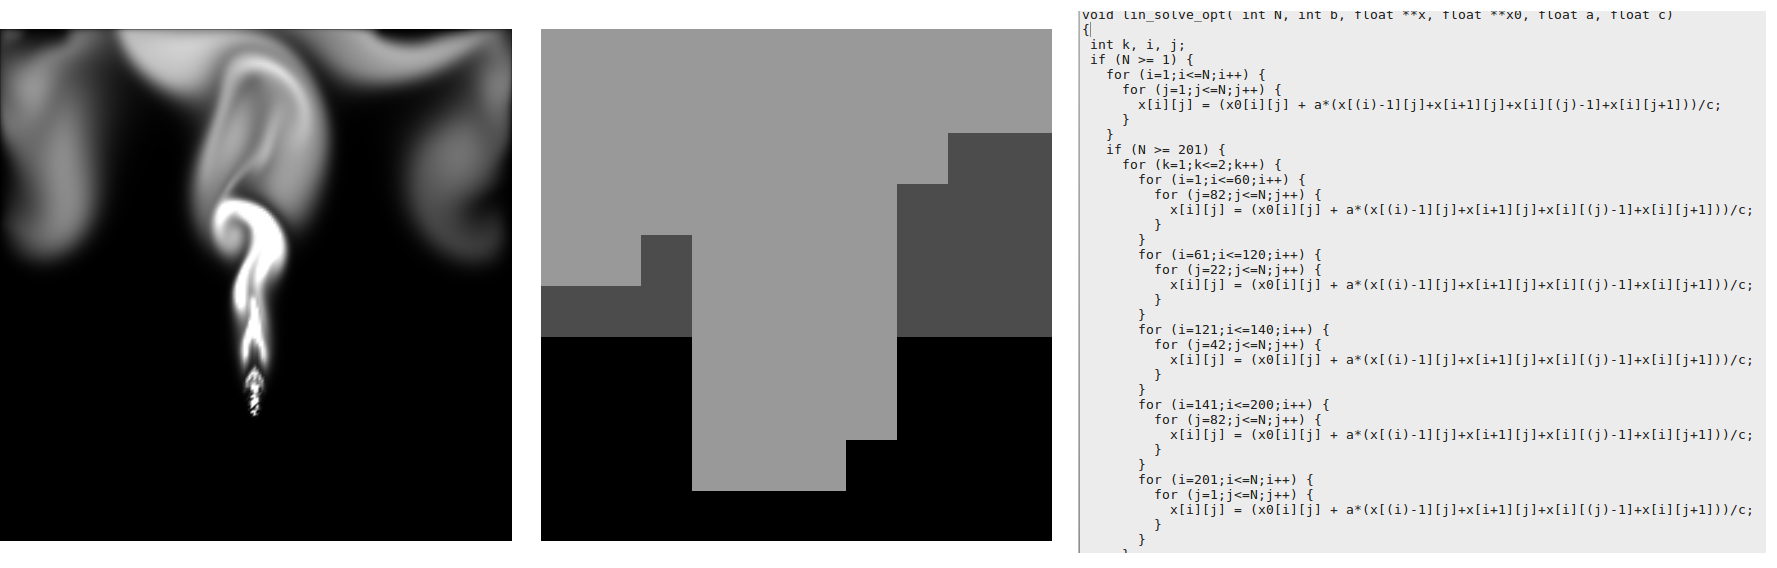
\includegraphics[scale=0.24]{img/ACR_pipeline.png}
\end{center}
\end{frame}
%~ %%%%%%%%%%%%%%%%%%%%%%%%%%%%%%%%%%%%%%%%%%%%%%%%%%%%%%%%%%%%%%%%%%%%%%%%%%%%%%%%
%~ \begin{frame}
%~ \frametitle{Refinamiento Adaptivo de Código}
%~ Se basa en: 
%~ \begin{itemize}
%~ \item \textbf{conocimiento especifico de dominio} 
%~ \begin{itemize}
%~ \item identificar regiones de complejidad
%~ \item asegurar buena presicion
%~ \item se codifican a traves de \lstinline{pragmas ACR}
%~ \end{itemize}
%~ \item \textbf{modelo poliedrico}: 
%~ \begin{itemize}
%~ \item transformaciones agresivas
%~ \item codigo eficiente
%~ \item \textcolor{red}{sujeto a su dominio de aplicacion}, excepto en la
%~ omision o modificacion de dependencias
%~ \end{itemize}
%~ \item \textbf{estrategia adaptiva}
%~ \begin{itemize}
%~ \item monitoreo constante de la ejecucion con una \textbf{cuadricula de estado}  
%~ \item generacion de codigo de forma dinamica
%~ \item utilizacion de \textbf{threads dedicados} al calculo y a la generacion de codigo
%~ \end{itemize}
%~ \end{itemize}
%~ \end{frame}
%%%%%%%%%%%%%%%%%%%%%%%%%%%%%%%%%%%%%%%%%%%%%%%%%%%%%%%%%%%%%%%%%%%%%%%%%%%%%%%%
\begin{frame}
\frametitle{Refinamiento Adaptivo de Código}
Componentes:
\begin{enumerate}
\item \textbf{Conocimiento Especifico de Dominio}
\item Monitoreo del Estado de Ejecucion
\item Generacion de Codigo Optimizado
\item Threads de Ejecucion
\end{enumerate}
\end{frame}
%%%%%%%%%%%%%%%%%%%%%%%%%%%%%%%%%%%%%%%%%%%%%%%%%%%%%%%%%%%%%%%%%%%%%%%%%%%%%%%%
\begin{frame}[fragile]
\frametitle{ACR: Conocimiento de Dominio}
\begin{columns}
\column[t]{0.40\textwidth}
\textbf{dominio de aplicacion}
\begin{itemize}
\item codigo + pragmas~embebidos
\item \textbf{satisface restricciones} del modelo poliedrico
\item \textbf{conocimiento de dominio} codificado por pragmas
\begin{itemize}
\item grid
\item monitor
\item alternative
\item strategy
\end{itemize}
\end{itemize}
\column[t]{0.57\textwidth}
\begin{block}{Codigo de Simulacion}
\begin{lstlisting}[basicstyle=\tiny,language=C]
while(true) {
  ...
  // lin_solve kernel
  #pragma ACR grid(10)
  #pragma ACR monitor(density[i][j], max, filtro)
  #pragma ACR alternative bajo(parameter, MAX = 1)
  #pragma ACR alternative medio(parameter, MAX = 3)
  #pragma ACR alternative alto(parameter, MAX = 4)
  #pragma ACR strategy direct(1, bajo)
  #pragma ACR strategy direct(2, medio)
  #pragma ACR strategy direct(3, alto)
  for (k = 0; k < MAX; k++) {
    for (i = 1; i <= N; i++) {
      for (j = 1; j <= N; j++) {
        lin_solve_computation(k, i, j);
      }
    }
  }
  ...
} 
\end{lstlisting}
\end{block}
\end{columns}
\end{frame}
%%%%%%%%%%%%%%%%%%%%%%%%%%%%%%%%%%%%%%%%%%%%%%%%%%%%%%%%%%%%%%%%%%%%%%%%%%%%%%%%
\begin{frame}[fragile]
\frametitle{ACR: Conocimiento de Dominio}
\begin{itemize}
\item \textbf{resolucion} de la cuadricula de monitoreo:
\begin{block}{}\lstinline{#pragma ACR }\textbf{grid}(\textit{tamaño}\lstinline{)}\end{block}
\item \textbf{porcion del estado} que vamos a monitorear:
\begin{block}{}\lstinline{#pragma ACR }\textbf{monitor}(\textit{datos}\lstinline{,} \textit{síntesis}\lstinline{[,} \textit{filtro}\lstinline{])} \end{block}
\item \textbf{calculo alternativo} para reemplazar codigo original: 
\begin{block}{}\lstinline{#pragma ACR }\textbf{alternative} \textit{nombre}\lstinline{(}\textit{tipo}\lstinline{,} \textit{efecto}\lstinline{)} \end{block}
\item \textbf{estrategias} de transformacion de codigo:
\begin{block}{}\lstinline{#pragma ACR }\textbf{strategy} tipo(p1, p2, ...) 
\begin{itemize}
\item dinamica: \lstinline{#pragma ACR strategy} \textbf{direct}(\textit{valor}\lstinline{,} \textit{alternativa}\lstinline{)} 
\item estatica: \lstinline{#pragma ACR strategy} \textbf{zone}(\textit{área}\lstinline{,}\textit{alternativa}\lstinline{)}
\end{itemize}
\end{block}
\end{itemize}
\end{frame}
%%%%%%%%%%%%%%%%%%%%%%%%%%%%%%%%%%%%%%%%%%%%%%%%%%%%%%%%%%%%%%%%%%%%%%%%%%%%%%%%
\begin{frame}[fragile]
\frametitle{ACR: Conocimiento de Dominio}
%~ \begin{itemize}
%~ \item \lstinline{#pragma ACR grid(}\textit{tamaño}\lstinline{)}
%~ \item \lstinline{#pragma ACR monitor(}\textit{datos}\lstinline{,} \textit{síntesis}\lstinline{[,} \textit{filtro}\lstinline{])}
%~ \item \lstinline{#pragma ACR alternative} \textit{nombre}\lstinline{(}\textit{tipo}\lstinline{,} \textit{efecto}\lstinline{)}
%~ \item \lstinline{#pragma ACR strategy direct(}\textit{valor}\lstinline{,} \textit{alternativa}\lstinline{)}
%~ \end{itemize}
\begin{columns}
\column[t]{0.74\textwidth}
\begin{block}{Kernel de Simulacion}
\begin{lstlisting}[basicstyle=\scriptsize,language=C]
// lin_solve kernel
#pragma ACR grid(10)
#pragma ACR monitor(density[i][j], max, filtro)
#pragma ACR alternative bajo(parameter, MAX = 1)
#pragma ACR alternative medio(parameter, MAX = 3)
#pragma ACR alternative alto(parameter, MAX = 4)
#pragma ACR strategy direct(1, bajo)
#pragma ACR strategy direct(2, medio)
#pragma ACR strategy direct(3, alto)
for (k = 0; k < MAX; k++) {
  for (i = 1; i <= N; i++) {
    for (j = 1; j <= N; j++) {
	  lin_solve_computation(k, i, j);
    } 
  }
}
\end{lstlisting}
\end{block}
\end{columns}
\end{frame}
%%%%%%%%%%%%%%%%%%%%%%%%%%%%%%%%%%%%%%%%%%%%%%%%%%%%%%%%%%%%%%%%%%%%%%%%%%%%%%%%
\begin{frame}
\frametitle{Refinamiento Adaptivo de Código}
Componentes:
\begin{enumerate}
\item Conocimiento Especifico de Dominio
\item \textbf{Monitoreo del Estado de Ejecucion}
\item Generacion de Codigo Optimizado
\item Threads de Ejecucion
\end{enumerate}
\end{frame}
%%%%%%%%%%%%%%%%%%%%%%%%%%%%%%%%%%%%%%%%%%%%%%%%%%%%%%%%%%%%%%%%%%%%%%%%%%%%%%%%
\begin{frame}[fragile]
\frametitle{ACR: Monitoreo del Estado de Ejecucion}
\begin{block}{}
ACR necesita obtener \textbf{informacion relevante} sobre la ejecucion
\begin{itemize}
\item para identificar regiones de diferente complejidad de calculo
\item generar codigo adecuado para cada region 
\item de forma \textbf{eficiente}, para no agregar costo computacional
\item resumida de forma regular, para permitir una representacion poliedrica
\end{itemize}
\end{block}
\begin{block}{}
Para ello, utilizamos una \textbf{cuadricula regular} 
\begin{itemize}
\item embebida en el espadcio de estado
\item cada celda representa una pocion (hiper-)cubica del estado
\end{itemize} 
\end{block}
\begin{block}{}
\textbf{Resolucion} y \textbf{Datos de Monitoreo}: \\
\lstinline{#pragma ACR }\textbf{grid}(\textit{tamaño}\lstinline{)} \\
\lstinline{#pragma ACR }\textbf{monitor}(\textit{datos}\lstinline{,} 
										\textit{síntesis}\lstinline{[,} 
										\textit{filtro}\lstinline{])} 
\end{block} 
\end{frame}
%%%%%%%%%%%%%%%%%%%%%%%%%%%%%%%%%%%%%%%%%%%%%%%%%%%%%%%%%%%%%%%%%%%%%%%%%%%%%%%%
\begin{frame}
\frametitle{ACR: Monitoreo del Estado de Ejecucion}
\begin{block}{Obtencion de Informacion}
\begin{enumerate} 
\item \textbf{filtro} de a valores  (opcional)
\item \textbf{sintesis} de informacion para cada celda
\item \textbf{agrupamiento} de celdas en \textbf{regiones de complejidad}
\end{enumerate}
\end{block}
\begin{center}
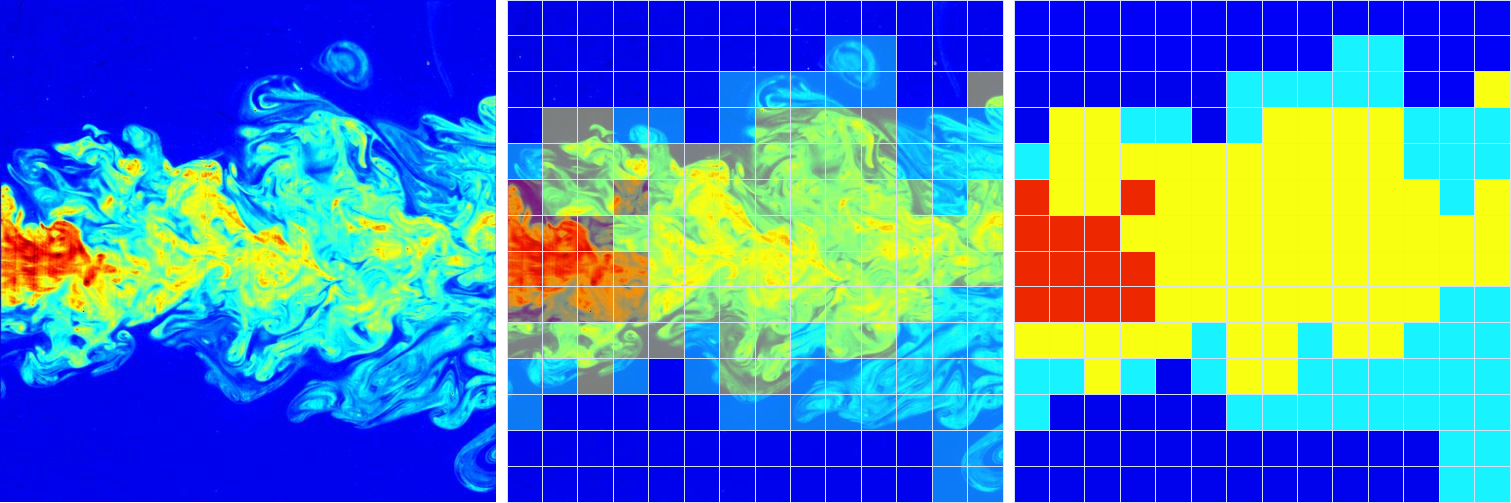
\includegraphics[scale=0.20]{img/turbulent_legal.png} 
\end{center}
%~ A cada region la representamos matematicamente con un \textbf{poliedro}
\end{frame}
%%%%%%%%%%%%%%%%%%%%%%%%%%%%%%%%%%%%%%%%%%%%%%%%%%%%%%%%%%%%%%%%%%%%%%%%%%%%%%%%
\begin{frame}[fragile]
\frametitle{ACR: Monitoreo del Estado de Ejecucion}
\begin{block}{pragmas}
\begin{lstlisting}[basicstyle=\scriptsize,language=C]
#pragma grid(14) 
#pragma monitor (presion[i][j],max,color)
int color(float val) {
  if      (val >= P_HIGH) return C_RED; 
  else if (val >= P_MED)  return C_YELLOW;
  else if (val >= P_LOW)  return C_CYAN;
  else                    return C_BLUE;
}
\end{lstlisting}
\end{block}
\begin{center}
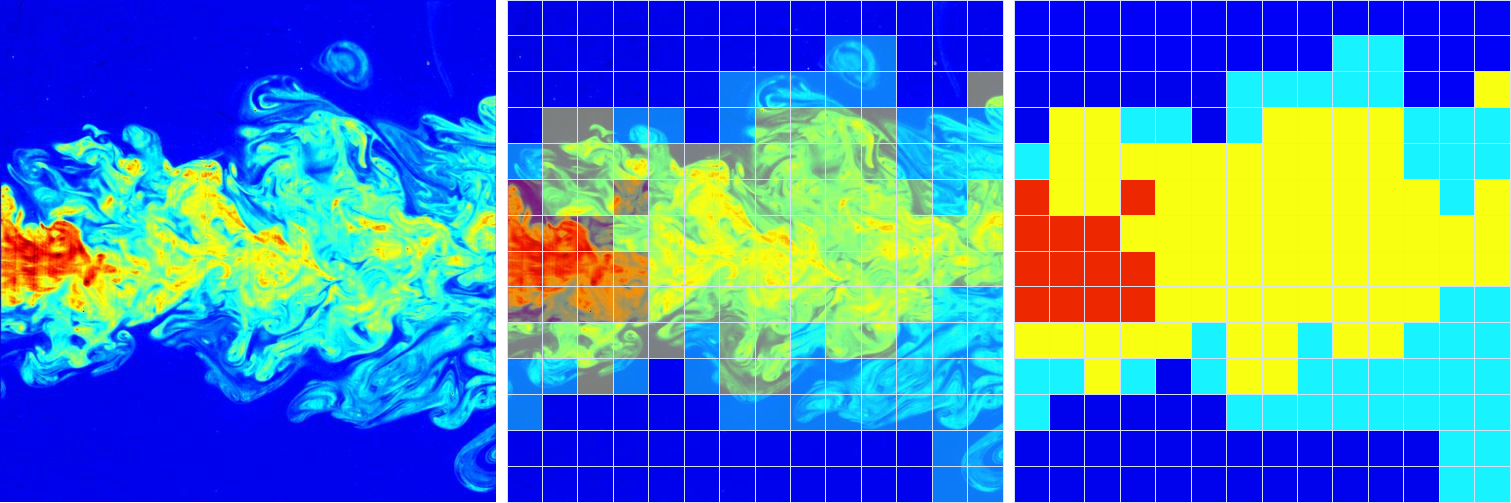
\includegraphics[scale=0.20]{img/turbulent_legal.png} \\
\end{center}
%~ A cada region la representamos matematicamente con un \textbf{poliedro}
\end{frame}
%%%%%%%%%%%%%%%%%%%%%%%%%%%%%%%%%%%%%%%%%%%%%%%%%%%%%%%%%%%%%%%%%%%%%%%%%%%%%%%%li
\begin{frame}
\frametitle{Refinamiento Adaptivo de Código}
Componentes:
\begin{enumerate}
\item Conocimiento Especifico de Dominio
\item Monitoreo del Estado de Ejecucion
\item \textbf{Generacion de Codigo Optimizado}
\item Threads de Ejecucion
\end{enumerate}
\end{frame}
%%%%%%%%%%%%%%%%%%%%%%%%%%%%%%%%%%%%%%%%%%%%%%%%%%%%%%%%%%%%%%%%%%%%%%%%%%%%%%%%
\begin{frame}
\frametitle{ACR: Generacion de Codigo Optimizado}
\begin{block}{al principio de la ejecucion}
\textbf{analisis} del kernel original con \textbf{Clan}
\end{block}
\begin{block}{Transformaciones Regulares}
luego de un cambio significativo en el estado:
\begin{enumerate}
\item aplicacion \textbf{estrategias de transformacion}
\begin{itemize}
	\item omitir calculos innecesarios
	\item usar bloques de codigo alternativost
\end{itemize}
\item \textbf{construir representacion poliedrica} de las regiones
\item \textbf{generacion de codigo} con Spot
\item \textbf{compilacion y reemplazo} del kernel que esta en ejecucion
\end{enumerate}
\end{block}
\end{frame}
%%%%%%%%%%%%%%%%%%%%%%%%%%%%%%%%%%%%%%%%%%%%%%%%%%%%%%%%%%%%%%%%%%%%%%%%%%%%%%%%
\begin{frame}[fragile]
\frametitle{ACR: signacion de Codigo}
\begin{columns}
\column{0.32\textwidth}
\begin{center}
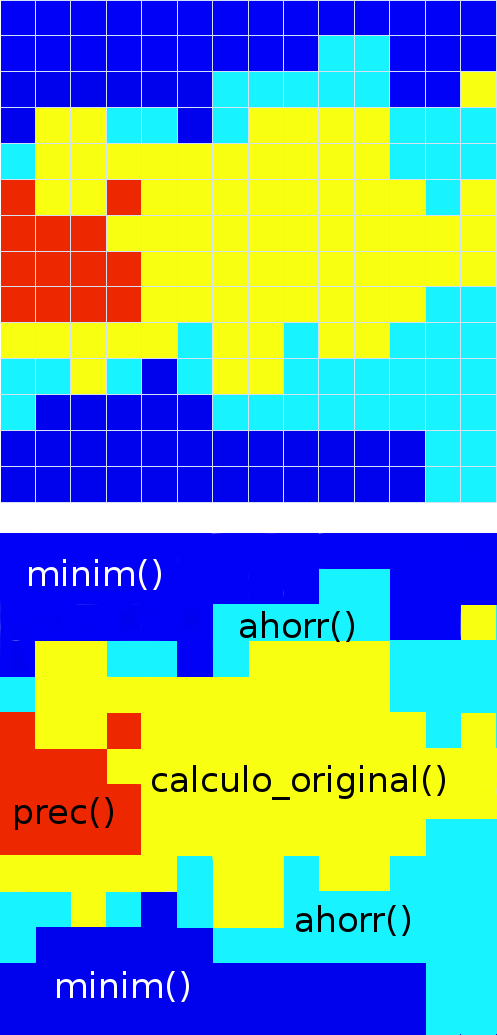
\includegraphics[scale=0.2]{img/asignacion_codigo.png}
\end{center}
\column{0.65\textwidth}
\begin{block}{}
\begin{lstlisting}[basicstyle=\scriptsize, language=C]
//kernel
for (int i = 0; i < N; i++)
  for (int j = 0; j < N; j++) 
    calculo_original(i,j);
\end{lstlisting}
\end{block}
\begin{block}{}
\begin{lstlisting}[basicstyle=\scriptsize]
// estrategias
#pragma strategy direct(C_RED, a1)
#pragma strategy direct(C_CYAN, a2)
#pragma strategy direct(C_BLUE, a3)
#pragma strategy zone
  ("i < N/14 and |j - N/2| < N/14", a1)
\end{lstlisting}
\end{block}
\begin{block}{}
\begin{lstlisting}[basicstyle=\scriptsize]
// codigo alternativo
#pragma alternatve a1(code, prec(i,j);)
#pragma alternatve a2(code, ahorr(i,j);)
#pragma alternatve a3(code, minim(i,j);)
\end{lstlisting}
\end{block}
\end{columns}
\end{frame}
%%%%%%%%%%%%%%%%%%%%%%%%%%%%%%%%%%%%%%%%%%%%%%%%%%%%%%%%%%%%%%%%%%%%%%%%%%%%%%%%
\begin{frame}
\frametitle{ACR: Asignacion de Codigo}
\begin{columns}
\column{0.32\textwidth}
\begin{center}
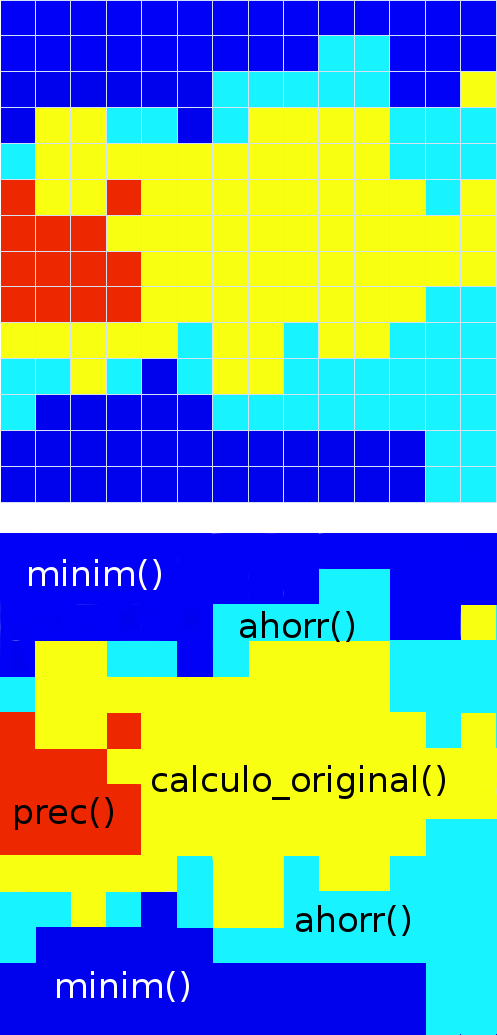
\includegraphics[scale=0.2]{img/asignacion_codigo.png}
\end{center}
\column{0.65\textwidth}
\begin{block}{propiedades del codigo generado}
\begin{itemize}
\item \textcolor{blue}{bajo costo de control}
\item \textbf{se corresponde biunivocamente} con su cuadricula
\item realiza calculos complejos \textbf{solo donde es necesario}
\item \textbf{mantiene las dependencias} lo mas posible
\end{itemize}
\end{block}
\end{columns}
\end{frame}
%%%%%%%%%%%%%%%%%%%%%%%%%%%%%%%%%%%%%%%%%%%%%%%%%%%%%%%%%%%%%%%%%%%%%%%%%%%%%%%%
\begin{frame}
\frametitle{Refinamiento Adaptivo de Código}
Componentes:
\begin{enumerate}
\item Conocimiento Especifico de Dominio
\item Monitoreo del Estado de Ejecucion
\item Generacion de Codigo Optimizado
\item \textbf{Threads de Ejecucion}
\end{enumerate}
\end{frame}
%%%%%%%%%%%%%%%%%%%%%%%%%%%%%%%%%%%%%%%%%%%%%%%%%%%%%%%%%%%%%%%%%%%%%%%%%%%%%%%%
\begin{frame}
\frametitle{ACR: Threads de Ejecucion}
\begin{block}{}
\textbf{alivianar sobrecarga de generacion}: 2 threads
\end{block}
\begin{block}{thread de calculo}
\begin{itemize}
		\item realiza \textbf{calculos intensivos}
		\item \textbf{monitorea} el estado de ejecucion
		\item \textbf{solicita} codigo optimizado
		\item \textbf{recibe y carga dinamicamente} codigo optimizado
		\item si las optimizaciones no son adecuadas, utiliza codigo original
\end{itemize}
\end{block}
\begin{block}{thread de generacion}
	\begin{enumerate}
		\item \textbf{recibe solicitudes} de generacion
		\item \textbf{genera y compila} codigo optimizado
		\item \textbf{responde las solicitudes}
	\end{enumerate}
\end{block}
\end{frame}
%%%%%%%%%%%%%%%%%%%%%%%%%%%%%%%%%%%%%%%%%%%%%%%%%%%%%%%%%%%%%%%%%%%%%%%%%%%%%%%%
\begin{frame}
\frametitle{ACR: Threads de Ejecucion}
\begin{center}
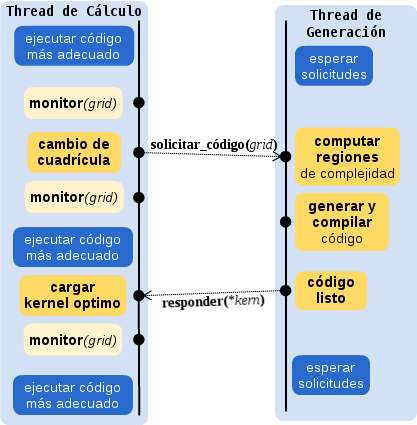
\includegraphics[scale=0.5]{img/threads_2.png}
\end{center}
\end{frame}
%%%%%%%%%%%%%%%%%%%%%%%%%%%%%%%%%%%%%%%%%%%%%%%%%%%%%%%%%%%%%%%%%%%%%%%%%%%%%%%%
\begin{frame} 
\frametitle{Contenido} 
\begin{enumerate}
\item Transformación de Código: Modelo Poliédrico
\item Herramienta estática: Spot
\item Refinamiento Adaptivo de Código
\item \textbf{Experimentos con Simulación de Fluidos}
\item Conclusiones y Trabajo Futuro
\end{enumerate}
\end{frame} 
%%%%%%%%%%%%%%%%%%%%%%%%%%%%%%%%%%%%%%%%%%%%%%%%%%%%%%%%%%%%%%%%%%%%%%%%%%%%%%%%
\begin{frame}
\frametitle{Caso de Estudio: Simulacion de Fluidos}
\begin{columns}
\column{0.60\textwidth}
	\begin{itemize}
		\item hola
	\end{itemize}
\column{0.40\textwidth}
\begin{center}

\includegraphics[scale=0.22]{img/saved_ssnapshot.png}
\end{center}
\begin{center}
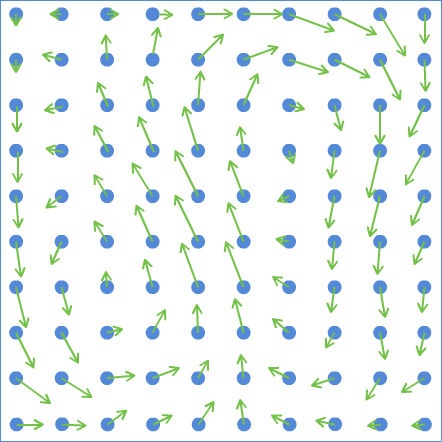
\includegraphics[scale=0.25]{img/particles_velocity.png}
\end{center}
\end{columns}
\end{frame}
%%%%%%%%%%%%%%%%%%%%%%%%%%%%%%%%%%%%%%%%%%%%%%%%%%%%%%%%%%%%%%%%%%%%%%%%%%%%%%%%





\begin{frame}
\frametitle{}

\end{frame}
%%%%%%%%%%%%%%%%%%%%%%%%%%%%%%%%%%%%%%%%%%%%%%%%%%%%%%%%%%%%%%%%%%%%%%%%%%%%%%%%


% end of slides
\end{document}
